\begin{table}[tb]
\centering
\caption{The main comparisons at label level: mean difference, 95\% interval over cohorts, labels and held-out cases, and the number of cohorts (datasets) with a positive mean. Modes are averaged per label except in the LoRA $-$ Dec sub-rows; LoRA $-$ Attn compares methods with the same head. VoCo covers three classification cohorts; pooled estimates are in Table~\ref{tab:cis}.}
\label{tab:key}
\renewcommand{\mci}[3]{#1\,{\scriptsize[#2, #3]}}\adjustbox{max width=\textwidth}{\small\setlength{\tabcolsep}{4pt}
\begin{tabular}{@{}lcccccccc@{}}
\toprule
 & \multicolumn{2}{c}{TAP-CT} & \multicolumn{2}{c}{SPECTRE} & \multicolumn{2}{c}{Pillar-0} & \multicolumn{2}{c}{VoCo} \\
\cmidrule(lr){2-3}\cmidrule(lr){4-5}\cmidrule(lr){6-7}\cmidrule(l){8-9}
Comparison & Mean [95\% interval] & $>0$ & Mean [95\% interval] & $>0$ & Mean [95\% interval] & $>0$ & Mean [95\% interval] & $>0$ \\
\midrule
\multicolumn{9}{@{}l}{\textit{Classification} (AUROC)} \\
LoRA $-$ Lin & \mci{$+0.032$}{$+0.007$}{$+0.053$} & 4/5 & \mci{$+0.037$}{$+0.009$}{$+0.075$} & 4/4 & \mci{$+0.033$}{$+0.021$}{$+0.044$} & 1/1 & \mci{$-0.071$}{$-0.168$}{$-0.005$} & 0/3 \\
LoRA $-$ Attn & \mci{$+0.022$}{$+0.006$}{$+0.042$} & 5/5 & \mci{$+0.033$}{$+0.003$}{$+0.078$} & 4/4 & \mci{$+0.034$}{$+0.021$}{$+0.052$} & 1/1 & \mci{$-0.031$}{$-0.145$}{$+0.043$} & 1/3 \\
Attn-only FT $-$ LoRA & \mci{$+0.019$}{$-0.001$}{$+0.054$} & 4/5 & \mci{$+0.002$}{$-0.037$}{$+0.026$} & 2/4 & \mci{$+0.001$}{$-0.002$}{$+0.004$} & 1/1 & \mci{$+0.036$}{$-0.024$}{$+0.102$} & 2/3 \\
Full FT $-$ Lin & \mci{$+0.022$}{$-0.061$}{$+0.068$} & 4/5 & \mci{$-0.117$}{$-0.195$}{$-0.059$} & 0/4 & \mci{$+0.004$}{$-0.013$}{$+0.021$} & 1/1 & \mci{$-0.034$}{$-0.136$}{$+0.027$} & 1/3 \\
Joint $-$ per-task & \mci{$+0.012$}{$-0.014$}{$+0.038$} & 3/5 & \mci{$-0.003$}{$-0.044$}{$+0.051$} & 3/4 & \mci{$-0.008$}{$-0.013$}{$-0.001$} & 0/1 & \mci{$-0.001$}{$-0.022$}{$+0.018$} & 2/3 \\
\addlinespace[2pt]
\multicolumn{9}{@{}l}{\textit{Segmentation} (Dice)} \\
Dec $-$ Lin & \mci{$+0.085$}{$+0.055$}{$+0.109$} & 5/5 & \mci{$+0.061$}{$+0.027$}{$+0.088$} & 5/5 & -- &  & \mci{$+0.680$}{$+0.433$}{$+0.746$} & 5/5 \\
LoRA $-$ Dec & \mci{$-0.005$}{$-0.021$}{$+0.024$} & 4/5 & \mci{$+0.023$}{$-0.018$}{$+0.076$} & 4/5 & -- &  & \mci{$-0.018$}{$-0.047$}{$+0.016$} & 2/5 \\
\quad per-structure models & \mci{$-0.021$}{$-0.036$}{$+0.002$} & 2/5 & \mci{$+0.006$}{$-0.003$}{$+0.031$} & 5/5 & -- &  & \mci{$-0.035$}{$-0.062$}{$-0.007$} & 0/5 \\
\quad joint models & \mci{$+0.011$}{$-0.021$}{$+0.066$} & 4/5 & \mci{$+0.040$}{$-0.039$}{$+0.147$} & 4/5 & -- &  & \mci{$0.000$}{$-0.034$}{$+0.047$} & 2/5 \\
Full FT $-$ Dec & \mci{$0.000$}{$-0.024$}{$+0.016$} & 4/5 & \mci{$-0.003$}{$-0.035$}{$+0.009$} & 2/5 & -- &  & \mci{$+0.015$}{$+0.007$}{$+0.023$} & 4/5 \\
Joint $-$ per-task & \mci{$-0.046$}{$-0.090$}{$-0.008$} & 0/5 & \mci{$-0.058$}{$-0.093$}{$-0.009$} & 0/5 & -- &  & \mci{$-0.041$}{$-0.081$}{$+0.004$} & 2/5 \\
\bottomrule
\end{tabular}
}
\end{table}

Table~\ref{tab:key} summarizes the main comparisons. Per-label and per-structure results are in Appendix~\ref{app:perlabel}, paired tests and further analyses in Appendix~\ref{app:paired}, seed repeats and controls in Appendix~\ref{app:revision}, and success and failure cases in Appendix~\ref{app:cases}.

\subsection{Classification: train the attention weights}
\label{sec:clsres}

\paragraph{Updating the encoder's attention weights beats both frozen probes.} On TAP-CT, SPECTRE and Pillar-0, LoRA raises held-out AUROC by $\numCiClsloralinAllMeandiff$ over the linear probe and by $\numCiClsloraattnAllMeandiff$ over the frozen attentive probe, which has the same head; both intervals exclude zero, and the gain over the attentive probe is positive in all \numCiClsloraattnAllClustersN{} cohort--backbone pairs (Table~\ref{tab:key}). Training the attention projections in full gains $\numCiClsattnftlinAllMeandiff$ and $\numCiClsattnftattnAllMeandiff$, again positive against the attentive probe in all \numCiClsattnftattnAllClustersN{} pairs. The gain comes from the encoder, not the head: the frozen attentive probe adds only $\numCiClsattnlinAllMeandiff$ to the linear probe. It is largest where the frozen probe is weakest ($\numGainbinLowMeandiff$ at a selection AUROC of at most 0.6, $\numGainbinTopMeandiff$ above 0.8; Figure~\ref{fig:gainprobe}), it survives the removal of FDG-PET/CT and COVID-CTset, where we did not rule out shortcuts ($\numCiClsloralinnoscAllMeandiff$), and LoRA is ahead of the linear probe in \numSeedsclsLoraLinAllPosN{} of \numSeedsclsLoraLinAllPairsN{} cohort--seed pairs of the repeated joint models.

\paragraph{Attention-only fine-tuning ranks best; LoRA comes close at about a fiftieth of the parameters.} Attention-only fine-tuning has the best mean rank over all slots (\numRankallAttnftMean{}; LoRA \numRankallLoraMean{}; Figure~\ref{fig:overview}c), ranks above LoRA on every backbone, and is ahead of LoRA in \numSeedsclsAttnftLoraAllPosN{} of \numSeedsclsAttnftLoraAllPairsN{} cohort--seed pairs, by $\numCiClsattnftloraAllMeandiff$ on average (interval $\numCiClsattnftloraAllLodiff$ to $\numCiClsattnftloraAllHidiff$), most on TAP-CT ($\numCiClsattnftloraTapctMeandiff$). LoRA reaches this accuracy while updating \numParamsbbTapctLora{} instead of \numParamsbbTapctAttnft{} encoder parameters on TAP-CT and \numParamsbbSpectreLora{} instead of \numParamsbbSpectreAttnft{} on SPECTRE.

\paragraph{The head is chosen first: on VoCo the linear head wins.} On VoCo the frozen attentive probe is behind the linear probe ($\numCiClsattnlinVocoMeandiff$), and every method that adapts the encoder under the attentive head inherits this deficit: against the attentive probe all eight are level (LoRA $\numCiClsloraattnVocoMeandiff$, attention-only fine-tuning $\numCiClsattnftattnVocoMeandiff$, full fine-tuning $\numCiClsfullftattnVocoMeandiff$), but against the linear probe they fall behind (LoRA $\numCiClsloralinVocoMeandiff$, most on FDG-PET/CT). Lin$\to$LoRA, which adapts the encoder under the linear head, is the best-ranked method on VoCo (\numVocorankLinThenLoragMean{}; Lin \numVocorankLinMean{}) and the one method with a positive mean difference to the linear probe on all four backbones ($\numCiClslinthenloraglinTapctMeandiff$ to $\numCiClslinthenloraglinSpectreMeandiff$; VoCo $\numCiClslinthenloraglinVocoMeandiff$). VoCo ran with the default settings of the other backbones.

\paragraph{Full fine-tuning needs its own setting.} With the default setting, Full FT is ahead of the linear probe on TAP-CT ($\numCiClsfullftlinTapctMeandiff$, and best on RSNA 2023 trauma, as \citet{liu2025anymc3d} found for spleen injury), level with it on Pillar-0 and VoCo, but does not train on SPECTRE: its median validation AUROC stays at \numTrajSpectrefullftLast{}, whereas attention-only fine-tuning at the same learning rates reaches \numTrajSpectreattnftLast{} (Figure~\ref{fig:fullftspectre}). With layer-wise learning-rate decay (0.75 per block), the best of three alternative settings on selection data, SPECTRE Full FT trains and is ahead of LoRA by $\numFixselSpectreLoraMeandiff$ (Table~\ref{tab:fullftfix}), a comparison that favors Full FT, as LoRA was not re-tuned.

\paragraph{Plain LoRA is enough.} No variant improves on LoRA on average: LoRA$_{\text{late}}$ changes held-out AUROC by $\numVsloraAllLoragMeandiff$, DoRA by $\numVsloraAllDoraMeandiff$, rsLoRA by $\numVsloraAllRsloraMeandiff$, LoRA+ABMIL by $\numVsloraAllBabmilMeandiff$ and the two-stage schedules by $\numVsloraAllLinThenLoragMeandiff$ and $\numVsloraAllAttnThenLoragMeandiff$; rsLoRA at a quarter of the learning rate, which matches its update scale to LoRA's, is level with LoRA on SPECTRE ($\numCtrlSpectreRsloraLowlrLoraMeandiff$) and Pillar-0 ($\numCtrlPillarZRsloraLowlrLoraMeandiff$) and behind on TAP-CT ($\numCtrlTapctRsloraLowlrLoraMeandiff$; Table~\ref{tab:controls}).

\subsection{Segmentation: a decoder on the encoder}
\label{sec:segres}

\paragraph{A multi-depth decoder on the frozen encoder gives most of the gain.} Replacing the linear probe by the frozen decoder raises Dice on every dataset and backbone, by $\numSegdeltaTapctLinDecMeandiff$ on TAP-CT, $\numSegdeltaSpectreLinDecMeandiff$ on SPECTRE and $\numCiSegdeclinVocoMeandiff$ on VoCo, whose deepest grid has one token per 48\,mm (Table~\ref{tab:key}). On TAP-CT this is all of LoRA's gain over the linear probe ($\numSegdeltaTapctLinLoraMeandiff$) and on SPECTRE most of it ($\numSegdeltaSpectreLinLoraMeandiff$). The pretrained weights matter: the TAP-CT architecture trained from a random initialization is behind fine-tuning of the pretrained encoder on every dataset, by $\numScratchLitsTapctMeandiff$ to $\numScratchTotalsegTapctMeandiff$ Dice (Table~\ref{tab:scratch}).

\begin{figure}[tb]
\centering
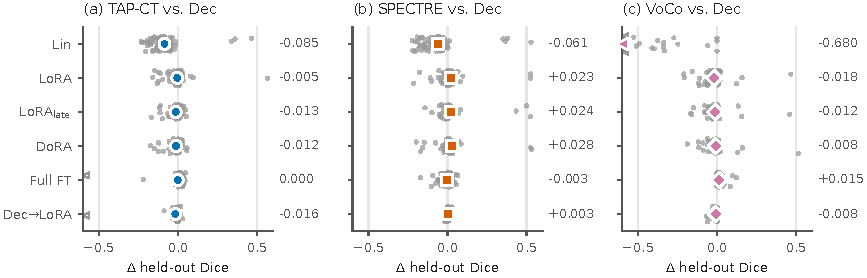
\includegraphics[width=\textwidth]{figures/fig_seg.pdf}
\caption{Segmentation: per-structure change in held-out Dice relative to the frozen decoder of the same backbone, dataset and mode, for (a) TAP-CT, (b) SPECTRE and (c) VoCo (grey: structure--mode pairs, triangles beyond the axis; colored: mean, printed on the right).}
\label{fig:seg}
\end{figure}

\paragraph{On top of the decoder, full fine-tuning ranks best and LoRA changes Dice little.} Full fine-tuning has the best mean rank (\numSegrankallFullftMean{}; LoRA \numSegrankallLoraMean{}; Figure~\ref{fig:overview}e), first on TAP-CT (\numSegrankTapctFullftMean{}) and VoCo (\numVocosegrankFullftMean{}), where it is ahead of the decoder by $\numCiSegfullftdecVocoMeandiff$ (interval $\numCiSegfullftdecVocoLodiff$ to $\numCiSegfullftdecVocoHidiff$); its mean change on TAP-CT is $\numSegdeltaTapctDecFullftMeandiff$ because \numSegdeltaTapctDecFullftDropN{} structure--mode pairs lose more than 0.1, among them the AMOS22 esophagus of the joint model ($\numSegdeltaTapctDecFullftMindiff$; Appendix~\ref{app:cases}). LoRA changes Dice relative to the frozen decoder by $\numCiSegloradecTapctMeandiff$, $\numCiSegloradecSpectreMeandiff$ and $\numCiSegloradecVocoMeandiff$ on TAP-CT, SPECTRE and VoCo, with intervals that include zero (Figure~\ref{fig:seg}); it gains most where the frozen decoder fails, in the SPECTRE AMOS22 joint model (\numSegAmosBBSpectreJointDec{} to \numSegAmosBBSpectreJointLora{}; Table~\ref{tab:segmodes}). Tripling the steps of the 15-structure joint models raised their Dice by $\numSegbudgetgainTapctMeandiff$ and $\numSegbudgetgainSpectreMeandiff$ (Table~\ref{tab:segbudget}), and \numConvSegAllLateBetter\% of segmentation runs selected one of their last two validations (Figure~\ref{fig:segconv}), so these comparisons rank methods at a fixed budget, not at convergence.

\begin{figure}[tb]
\centering
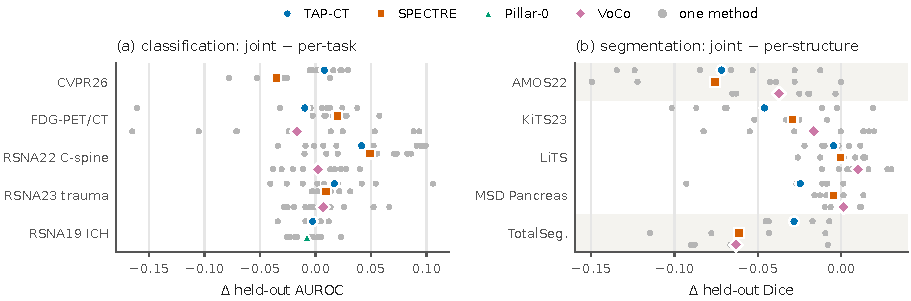
\includegraphics[width=\textwidth]{figures/fig_joint_main.pdf}
\vspace{-14pt}
\caption{One model per dataset against one model per label. (a) Joint minus per-task held-out AUROC per classification cohort and (b) joint minus per-structure held-out Dice per segmentation dataset; large markers: mean over methods and labels (structures) per backbone; grey dots: individual methods. Per-label values are in Appendix~\ref{app:perlabel} and Figure~\ref{fig:joint}.}
\label{fig:jointmain}
\end{figure}

\subsection{One model per dataset or one per label}
\label{sec:jointres}

\paragraph{In classification, one model per cohort is on average level with one per label, at a fraction of the training.} Joint minus per-task AUROC is $\numCiClsjointAllMeandiff$ on TAP-CT, SPECTRE and Pillar-0 (interval $\numCiClsjointAllLodiff$ to $\numCiClsjointAllHidiff$) and $\numCiClsjointVocoMeandiff$ on VoCo ($\numCiClsjointVocoLodiff$ to $\numCiClsjointVocoHidiff$), while a joint model uses $1/K$ of the training steps of the $K$ per-label models it replaces; per cohort, averaged over methods, the difference ranges from $\numJointdeltaMin$ to $\numJointdeltaMax$ (Figure~\ref{fig:jointmain}a; per method in Figure~\ref{fig:joint}).

\paragraph{In segmentation, the cost of one joint model lies in small structures and in the budget per structure.}\label{sec:jointseg} One joint model per dataset changes Dice by $\numCiSegjointTapctMeandiff$, $\numCiSegjointSpectreMeandiff$ and $\numCiSegjointVocoMeandiff$ on TAP-CT, SPECTRE and VoCo, most on the 15-structure AMOS22 (Figure~\ref{fig:jointmain}b). Much of this comes from \numSegcollapseN{} of \numSegcollapseCellsN{} structure--method pairs on small structures (adrenal glands and esophagus of AMOS22, merged glands of TotalSegmentator), where the joint model scores below 0.01 Dice; without them the mean over structure--method pairs moves from $\numSegjointTapctMeandiff$ to $\numSegjointTapctNocollapseMeandiff$ on TAP-CT and from $\numSegjointSpectreMeandiff$ to $\numSegjointSpectreNocollapseMeandiff$ on SPECTRE. At matched total compute, the joint LoRA model is ahead of per-structure LoRA models on both 15-structure datasets and both backbones ($\numCmTotalsegSpectreLoraJointdiff$ to $\numCmAmosBBSpectreLoraJointdiff$ Dice), whereas with the frozen decoder and full fine-tuning it is behind in three of the four pairs (Table~\ref{tab:segcm}).
